\section{Study region}
Douala is the economic capital of Cameroon located at 04\textdegree03'N 9\textdegree41'E in Central Africa with a high population over 3 million inhabitants\cite{populationstatdouala2021}(Fig.\ref{fig:douala_city_map}). The problem of flooding is widespread in Cameroon\cite{bruckmann2019analyse,tangan2018community}. For instance, floods events have occurred up to 5-10 times a year in the capital and 1-5 times a year in rural areas such as Maga and Lagdo (Northern region)\cite{tangan2018community}. Since 1975, when the Bamendjin dam was constructed, the Ndop plain in northeastern Cameroon has experienced periodic flooding, especially during the rainy season\cite{sighomnou2005cameroon}. Limbe, a seaside town in the southwest region of Cameroon, was also heavily flooded in 2001, with over 2000 people homeless, and destroyed properties and infrastructure\cite{ngalim2020stakeholders}. In 2008, the geographical area of Nkolbisson, Cameroon, for example, was hit by two catastrophic floods\cite{bruckmann2019analyse,tangan2018community}. 
\begin{figure}[hbt!]
	\centering
	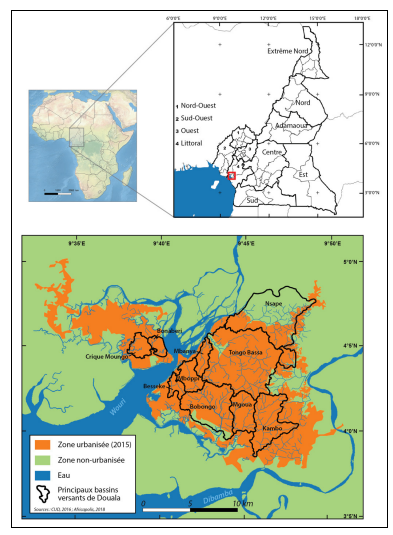
\includegraphics[width=0.8\linewidth]{figure/douala_city_map.png}
	\caption{Location of the urban area and the main watersheds of Douala. (Source: Figure 5 from \cite{bruckmann2019analyse})}
	\label{fig:douala_city_map}
\end{figure}

\subsection{Flood triggering mechanisms in Cameroon}

Poor waste management has been identified as a major cause of flooding in developing countries like Cameroon\cite{barthelemy2016legislative}. In Mefou, in central Cameroon and in the Dakar district of Douala (Fig.\ref{fig:dechet}), drains were observed to be clogged with plastic bottles and other solid waste\cite{gideonrole}. In another study by \cite{wung2019enhancing}, flooding in Limbe was discovered to be resulted from river channel blockage caused by indiscriminate dumping of refuse into the waterway and sediment deposition from upstream.

\begin{figure}[hbt!]
	\centering
	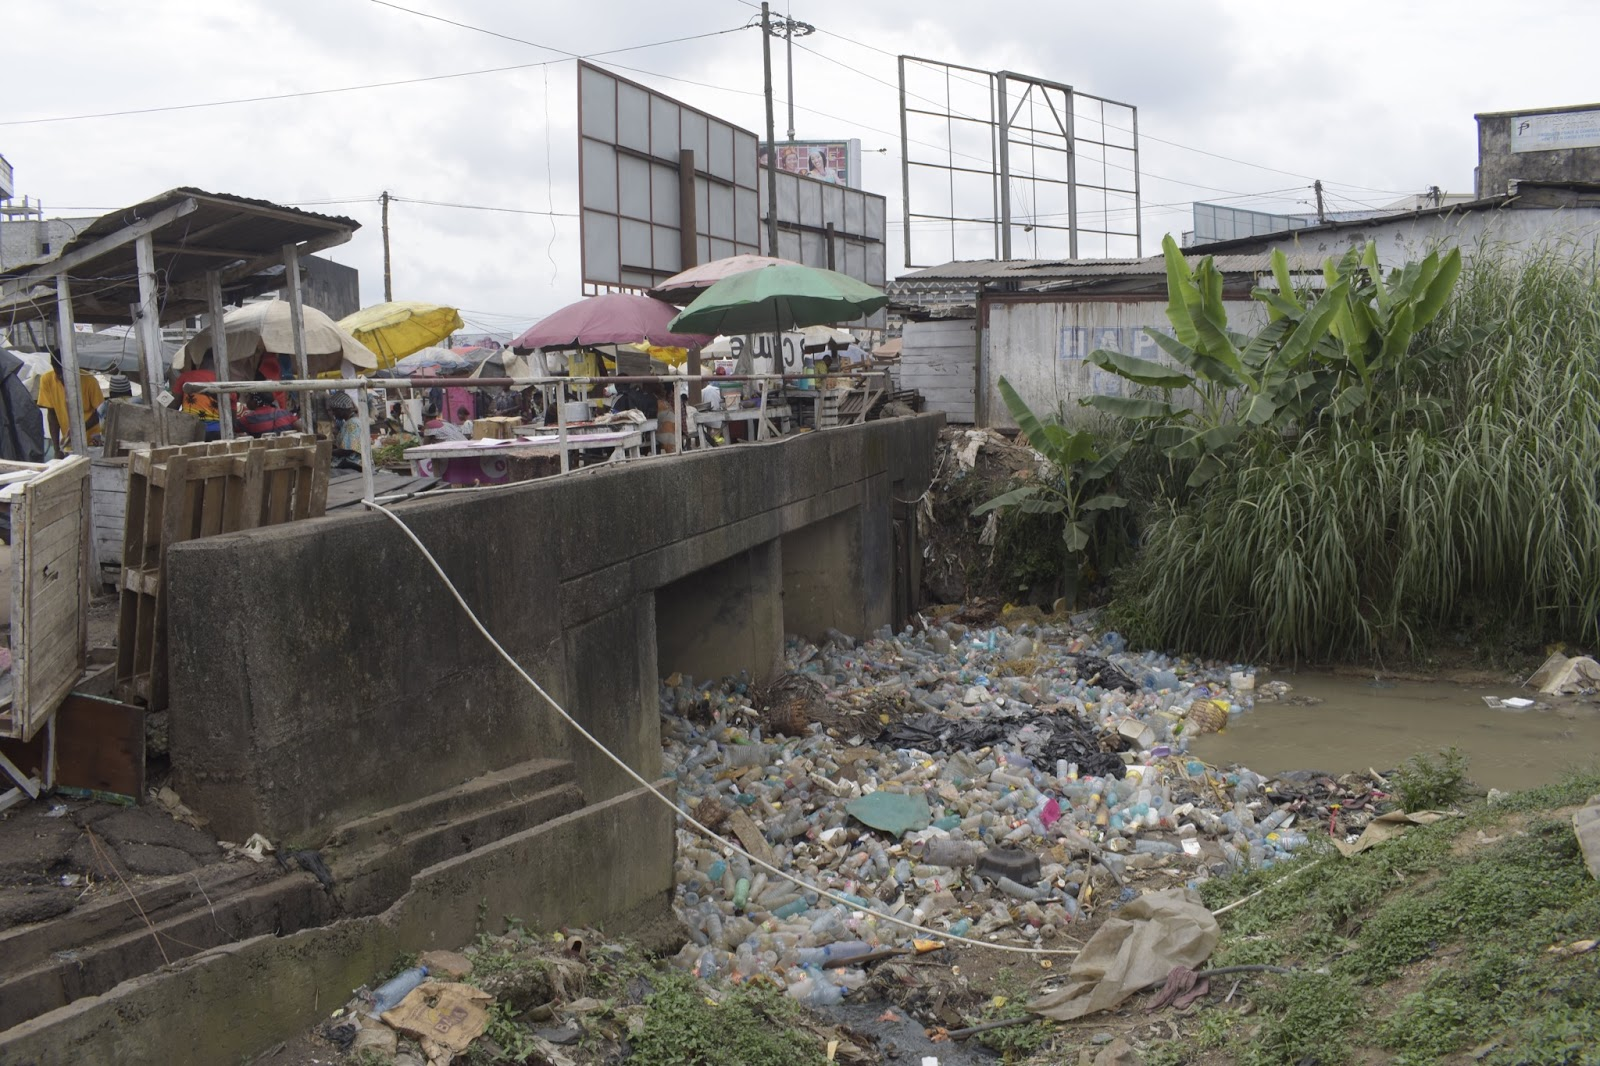
\includegraphics[height=4cm,keepaspectratio,width=0.8\linewidth]{figure/dechet.JPG}
	\caption{Plastic pollution completely blocking a waterway in the Dakar district of Douala, Cameroon\cite{greenpeaceorg}
}
	\label{fig:dechet}
\end{figure}

In the context of climate change, the increasing urbanization of the region is known to disregard drainage systems designed to contain runoff and the maximum volume of water that must flow through them during rainy periods. Thus, factors such as inadequate drains, uncontrolled waste disposal, and the nature of precipitation were considered common and important triggers to consider in mitigating and preparing for flooding in the region\cite{ngalim2020stakeholders}. 

\subsection{Precipitation in Douala}
In Douala, flooding is common during the rainy season from March to October(Fig.\ref{fig:douala_city_map} and \ref{fig:climateprecipitation}). The Tongo Bassa watershed located in the heart of the great Cameroonian economic metropolis of Douala, is one of the most affected urban location of the city. Tongo Bassa occupies an area of approximately 4200 ha or 42 $km^2$. The Tongo Bassa basin is crossed by three rivers and is characterized by a gentle slope (0.1 to 0.7\%) which exposes it to the daily tide variations. Bonamoussadi, Bepanda and Makepe Missoke are the most frequently affected areas, distributed on both sides of the Tongo Bassa river. 

\begin{figure*}[hbt!]
	\centering
	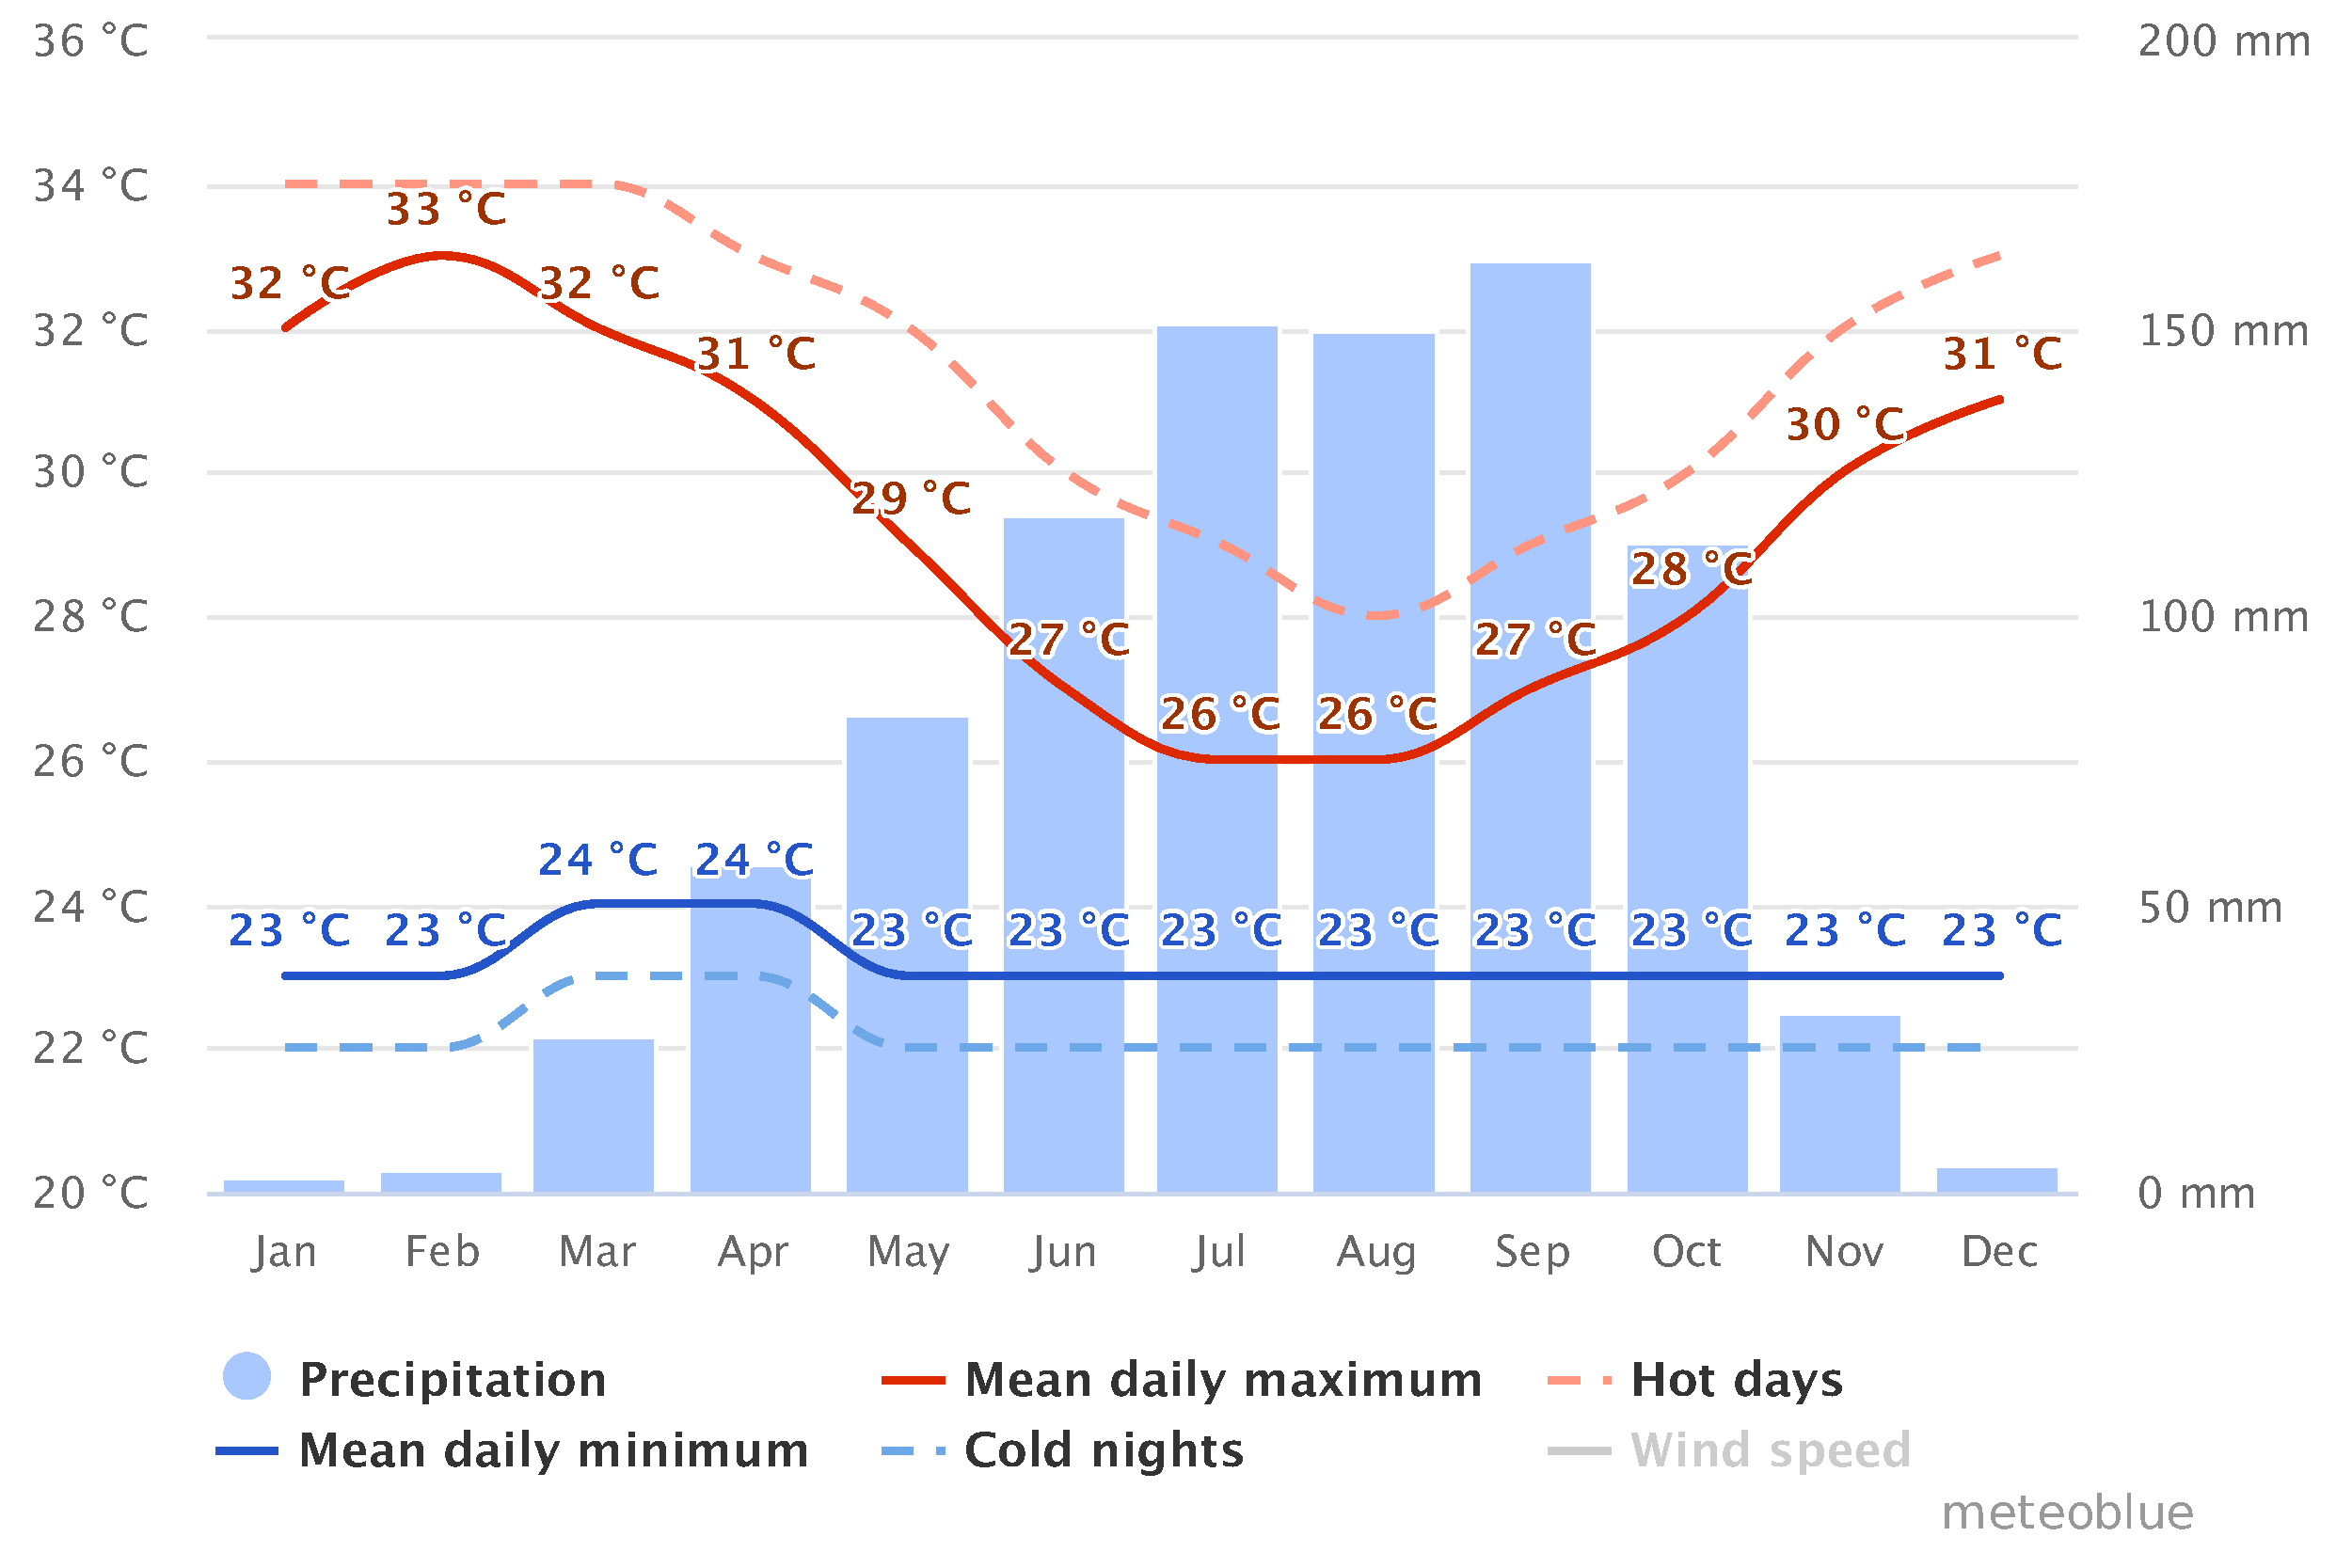
\includegraphics[width=0.5\linewidth]{figure/douala_climate.pdf}
	\caption{Douala Average temperatures and precipitation (Littoral, Cameroon, 4.05°N 9.7°E)(Source: www.meteoblue.com)\cite{meteoblue}. The mean daily maximum (solid red line) shows the maximum temperature of an average day for every month for Douala. Likewise, mean daily minimum (solid blue line) shows the average minimum temperature. Warm days and cool nights (dashed red and blue lines) show the average of the hottest day and coldest night of each month of the last 30 years}
	\label{fig:climateprecipitation}
\end{figure*}
\begin{figure}[hbt!]
	\centering
	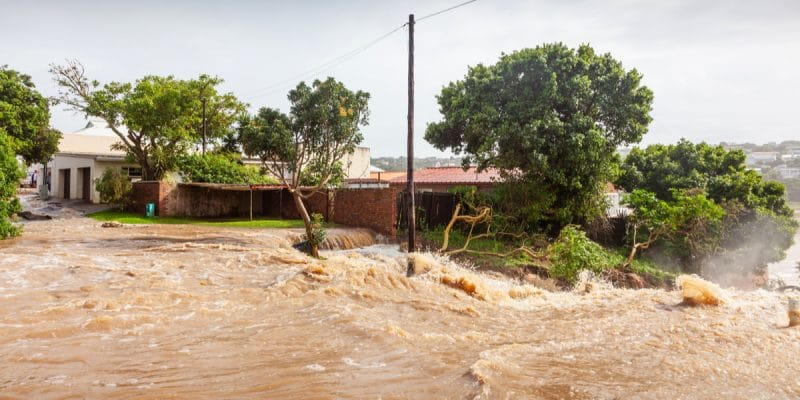
\includegraphics[width=0.8\linewidth]{figure/douala.jpg}
	\caption{Douala floods are frequents in July and August with several damage\cite{Afrik21}}
	\label{fig:floodimage}
\end{figure}

This highly urbanized basin is subject to rapid runoff towards low-lying areas with limited infiltration and high sedimentation rate in drains. Floods in these areas frequently affect residential houses, goods and services due to their exposure and low coping capacities of inhabitants, causing damage and loss of lives. This case is pertinent to the following dates: August 2\textsuperscript{nd} to 3\textsuperscript{rd}, 2000, August 9\textsuperscript{th}, 2010, and more recently that of August 21\textsuperscript{st}, 2020, August 11\textsuperscript{th}, 2021, September 1\textsuperscript{st}, 16\textsuperscript{th} and 18\textsuperscript{th} 2021.

\begin{figure}[hbt!]
	\centering
	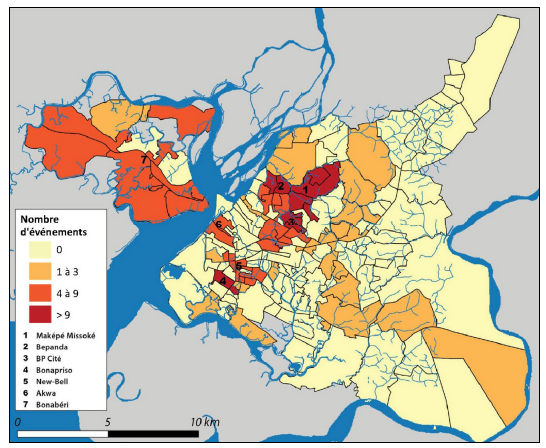
\includegraphics[width=0.8\linewidth]{figure/flood_distribution1984_2018.png}
	\caption{Spatial distribution of floods (31 events recorded) in Douala districts over the period 1984-2018. (Source: Figure 5 from \cite{bruckmann2019analyse})}
	\label{fig:flood_distribution1984_2018}
\end{figure}


\section{Methods}

\subsection{Synthetic Aperture Radar}
Synthetic Aperture Radar (SAR) is an active microwave remote sensing system in which a sensor sends a beam towards the ground and acquires the backscattered signals after interacting with the Earth's surface. Unlike optical satellite imagery, it is independent of solar electromagnetic energy and can capture high-resolution images during the day and night, in almost all-weather conditions, and through clouds \cite{Landuyt2019,WANG1995324}.

The scattering of objects on the SAR image is highly influenced by the terrain (geometry, features, etc.) and also acquisition properties (resolution, incident wave, ascending or descending-pass, etc.). In addition, the acquisition can be done by emitting and receiving horizontal (H) or vertical (V) polarization(cross-polarized (VH/HV) or co-polarized (HH/VV) acquisitions) that interacted differently with the ground. It therefore provides an additional information to characterize the phenomena of the observed region\cite{WANG1995324}. The best accuracy for flood mapping has been reported to be by using VH polarization configuration\cite{carreno2019flood}.

For a given mission of constant incidence angle and wavelength, the backscattering signal for a targeted area varies depending on the dielectric properties of the target, the physical shape of the scatterers in the target area of the resolution cell\cite{farr1993radar}. Water and metals represent objects with higher dielectric content than other materials and have a very large response. Therefore, if the geometric shape lies in front of the signal line of sight (such as the roofs of houses), the objects will appear bright because a strong signal is returned (or backscattered) to the sensor. On the other hand, if the surface is flat as a plane mirror, the incoming pulses reflect away from the sensor and they appear as a dark feature (flat water, etc.). Irregular geometries, such as vegetation cover, are grayed out because scattering occurs in all directions and only a small fraction of signals is reflected back to the sensor. Thus before flooding occurs, dry soil or vegetation would have a lower dielectric response. After an area has been flooded ,due to the high dielectric constant of water (80), the moisture content increases the returned signals. This response presents multiple reflections possibilities(specular reflection, double bounce, etc.) from the surface, which can make it difficult to extract the flood map, especially in vegetated (specular reflection or double-bounce within canopy) and urban areas (double bounce in buildings).

The SAR image has two major inherent limitations due to its angular viewing that leads to radiometric distortions or foreshortening and the diffraction induced speckle noises. SAR data exhibited salt and pepper noise are caused by a phenomenon inherent in the active coherent illumination system called speckles. These speckles are due to random constructive and destructive interferences in each resolution cell of the image, resulting in degradation of image quality and interpretation. Thus, before any application, these radar images must be pre-processed to remove the noises either by spatial filtering or by multi-looking operations\cite{argenti2013tutorial}.

In general, floods occur under severe weather conditions with heavy rainfall and dense cloud cover. These clouds hinder the effectiveness of optical satellite imagery\cite{sanyal2004}, hence, the use of SAR data for flood monitoring has become very common\cite{rao2006advantage}, and much research has demonstrated its effectiveness in flood events assessment \cite{martinez2007mapping}.

SAR-based flood detection techniques comprise thresholding-based methods \cite{Inglada2007}, image segmentation \cite{martinis2009towards}, statistical active contouring \cite{horritt2001flood}, rule-based classification \cite{pradhan2016new}, interferometric-SAR coherence analysis and data fusion approaches \cite{d2016bayesian}. 
To improve accuracy, thresholding-based flood detection techniques have evolved by merging additional data with the topographic data.


\subsection{Change detection}
The United Nations Platform for Space-based Information for Disaster Management and Emergency Response (UN-SPIDER) has made available an advanced thresholding-based method that generates flood extent map and assessment of affected areas\cite{un-spider}. 

The extent of a flood event is calculated using Sentinel-1 SAR data and a change detection method. This tool also includes an assessment of the number of people likely to be exposed, cropland and metropolitan areas affected, which can be cross-referenced with the generated flood extent layer and visualized in minutes.
This approach is suitable for developing countries as it uses the Google Earth Engine (GEE) cloud computing platform (https://code.earthengine.google.com) to process cloud-based remote sensing data. The main advantage is the speed of the computation, which is outsourced to Google's servers, as well as the availability of a variety of regularly updated datasets that are accessible directly in the code editor. Thus, it is possible to access the satellite data archive without having to download the raw data. The GEE GRD imagery includes the following steps: thermal noise removal, radiometric calibration, terrain correction. Therefore, only a speckle filter needs to be applied during pre-processing. 

A change detection approach was chosen, where images before and after the flood event are compared. This is due to the difficulties of detecting the city of Douala, which is mainly composed of vegetation and a dense urban area.  Using the basic histogram thresholding method, it is therefore difficult to distinguish flooded vegetation from urban flooding due to double-bounce backscatter\cite{manavalan2018review}.

Several supplemental datasets are used to suppress false positives in the flood extent layer. The European Commission's Joint Research Centre Global Surface Water dataset ('Source: EC JRC/Google', https://global-surface-water.appspot.com/) is used to mask all areas covered by water for more than 10 months per year with a spatial resolution of 30 m\cite{pekel2016high}. 

To eliminate pixels with slopes greater than 5\%, the Hydrological data and maps based on SHuttle Elevation Derivatives at multiple Scales (HydroSHEDS) digital elevation model of 3 Arc-Seconds was used. 
%\begin{figure*}[hbt!]
%	\centering
%	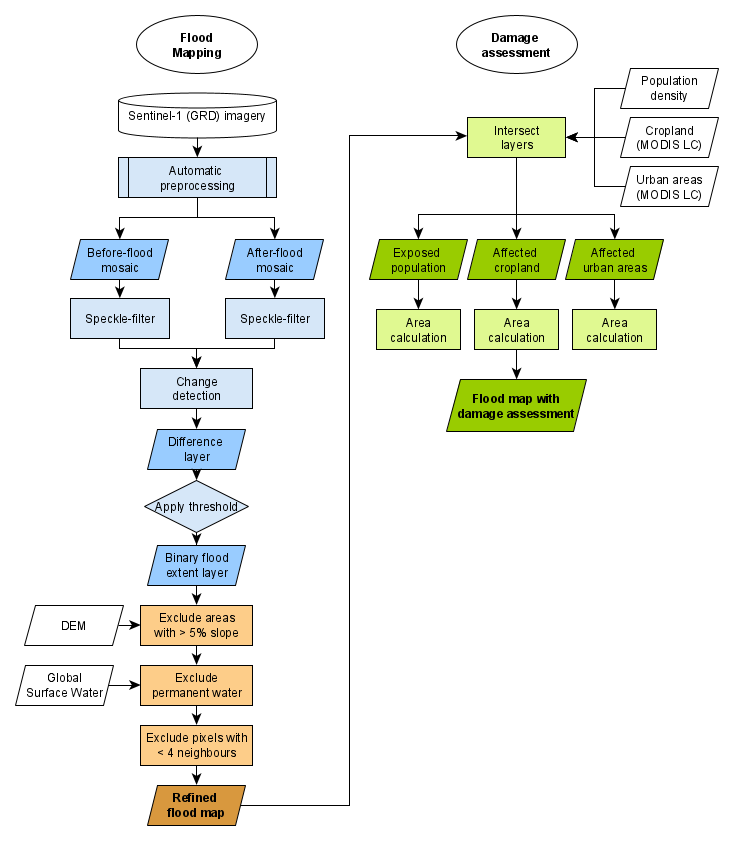
\includegraphics[width=0.6\linewidth]{figure/flood_mapping_GEE_workflow_1.png}
%	\caption{ The UN-SPIDER Recommended Practice workflow for flood mapping and damage assessment using Sentinel-1 SAR data in Google Earth Engine (Source:UN-SPIDER)\cite{un-spider}}
%	\label{fig:flood_mapping_GEE_workflow_1}
%\end{figure*}

\subsection{Sentinel 1}
Sentinel-1 is part of the space missions by the European Union and carried out by the European Space Agency (ESA) under the Copernicus program\cite{Panetti2014,geudtner2014sentinel}. This program aims to establish a global, continuous, autonomous, high quality and wide-range Earth observation capability. 

The constellation of polar-orbiting Sentinel-1 satellites (Sentinel-1A and Sentinel-1B) provides continuous SAR data day and night with a revisit time of 6 days. The data provided by the Copernicus Open Access Hub are mainly Single Look Complex (SLC) used for interferometry and the Ground Range Detected (GRD)\cite{filipponi2019sentinel}. Sentinel-1 Level 1 GRD products consist of focused SAR data that are multi-looked and projected to ground range using an Earth ellipsoid model. These data are accessible via the GEE and were used to map a flood event in August 2020, in Douala.
Sentinel-1 in the GEE are provided in different polarizations, modes, passes and resolutions\cite{ gees1}:
\begin{enumerate}
    \item Transmitter Receiver Polarization: ["VV"], ["HH"], ["VV", "VH"], or ["HH", "HV"]
    \item Instrument Mode: "IW" (Interferometric Wide Swath), "EW" (Extra Wide Swath) or "SM" (Strip Map). 
    \item Orbit Properties pass: "ASCENDING" or "DESCENDING"
    \item Spatial resolution meters: 10, 25 or 40
    \item GRD resolution: "M" (medium) or "H" (high).
\end{enumerate}
The Sentinel 1 satellite acquired were single polarization data at a spatial resolution of 5 m × 20 m, a 250 km swath width of view and in VH polarization.
\subsection{Twitter}

Publicly available tweets are retrieved by using python libraries snscrape (https://github.com/JustAnotherArchivist/snscrape). In this study, we used two different keywords in the query – "Cameroon flood" and "Cameroun inundation" (French for "Cameroon flood" ). For each tweet, we extract and retain the following information: tweeted time, content, number of replies, number of retweets, and number of likes. The tweets retrieved include both original tweets and replies, but not retweets. This work reports and discusses only aggregated statistics of the tweets.

To retrieve useful common terms and conduct sentimental analysis of the tweets, we need to pre-process the content of the tweets using techniques in Natural Language Processing. Natural Language Toolkit (NLTK) python library was used to perform the following steps:
\begin{enumerate}
    \item Remove links, mentions, and hashtag
    \item Splitting sentences into words and punctuation marks, or tokenization
    \item Remove stopwords such as articles, prepositions, and punctions that does not contribute to the meaning of the content
    \item Reducing the words into a root form or lemmatization, i.e. convert 2nd and 3rd forms of the verbs to the base verb
    \item Remove non-alphabetical characters and keep only words that contain three or more letters
\end{enumerate}

Using processed content from the tweets, we can determine the most common terms by using tf-idf vectorization. Term frequency of term t in document d is defined as:
\begin{equation}
tf(t,d)=n/N
\end{equation}

where n is the frequency of the term t in document d and N is the frequency of the term t in all documents in the database of the library used. The inverse document term frequency is given by:
\begin{equation}
tdf(t,d)=log(\frac{D}{d\in D: t \in D})
\end{equation}

where D is the total number of documents and ${d\in D: t \in D}$ represents the number of documents in which we find the term t. The product of term frequency and inverse document term frequency is called tf-idf. A more common term would have the tf-idf value of closer to zero. In our analysis, tf-idf vectorization using a machine learning python library, scikit-learn. Word clouds are then generated based on tf-idf values.

To conduct sentimental analysis, we use a python library Textblob. This library contains a trained models that could determine the polarity and subjectivity of a given text. Polarity ranges between -1 and 1 with positive values reflecting emotionally positive message and negative values reflecting emotionally negative messages. Those that are neutral would have polarity of 0. Subjectivity ranges between 0 and 1 with 1 being subjective and 0 being objective. Using both polarity and subjectivity would allow us to evaluate the sentiments of twitter users toward flooding issues in Cameroon.
